\documentclass[10pt]{article}

%%%%%%%%%%%%%%%%%%%%%%%%%
% Package configuration %
%%%%%%%%%%%%%%%%%%%%%%%%%

% Page margin
\usepackage[margin=1in]{geometry}

% Support for bold small cap font
\usepackage[tuenc]{fontspec}%for lualatex case
\setmainfont{CMU Serif}

% Better typesetting quality
% also used to customize section style
\usepackage{microtype}

% Redefine section, subsection styles
\usepackage[compact,center,explicit]{titlesec}
\usepackage{textcase}
\titleformat{\section}{\scshape\lsstyle\normalsize\filcenter}
    {\thesection}{1em}{\textls{\MakeTextUppercase{#1}}}
\titleformat{\subsection}{\normalfont\small\bfseries\filcenter}
    {\thesubsection}{1em}{#1}

% Setup link
\usepackage{hyperref}
\hypersetup{colorlinks,breaklinks,citecolor=blue}

% Set up biblatex database
\usepackage[
    %style=authortitle-tcomp,
    %firstinits=true,
    %backref=true,
    natbib=true,
    backend=biber,
    % NOTE: This options ensures that no automatic et al. is generated
    maxbibnames=99,
    % NOTE: This option must be enabled with 'babel' package
    useprefix=false
]{biblatex}
\addbibresource{umd_phd_candidacy_paper.bib}

%%%%%%%%%%%%%%%%%
% User settings %
%%%%%%%%%%%%%%%%%

% User-defined variables
\def\BaBar/{\textsc{BaBar}}

% Title info
\title{Review on Testing lepton flavor universality in semileptonic channels}
\author{Yipeng Sun}
\date{\today}

\begin{document}
\maketitle

\section{Introduction}
What is LFUV? (FU physics, FUV physics)
Why semileptonic decays (good thing about form factor)?
A historical review, starting from 2012 BaBar;
Talk about Phoebe's run 1 analyses.
Talk about what we are doing.
Talk about expected improvements and drawbacks of our upcoming analysis compared
to run 1.

\section{Theory}
\subsection{Lepton flavor universality}

\subsection{Advantages of semileptonic channel decays}

\subsection{Higgs mechanism}

\subsection{2-Higgs doublet models (2HDM)}
% type-II model claimed to be excluded; type-III (very similar to type-II) still
% alive.

\subsection{Leptoquark models}


\section{Review of colliders/detectors for $B$-physics}
One may ask: Why are we so interested in $B$ mesons?
% Initially B factories are meant for CP violation detection.
Initially, B factories, such as \BaBar/, was primarily constructed to do
precision measurements on CP violation of \cite{Luth:1994}.


% Talk about why B-bound states/mesons are also good for testing LFUV.
$B$ mesons provide a good testing bed for new physics:
They have enough energy to decay into all 3 flavors of leptons;
at the same time, they are not too heavy to produce.

All measurements start from $b\bar{b}$ bound states.
Electron-position colliders\footnote{
    Such as PEP-II, the collider for the \BaBar/ experiment.
} produce $\Upsilon_{4s}$ via electroweak interaction
Hadron colliders\footnote{
    Such as Large Hadron Collider (LHC) for the LHCb experiment.
} produce $\Upsilon_{4s}$ via strong interaction.


% Talk about PEP-II and its asymmetrical beam energies
PEP-II is an asymmetrical $e^- e^+$ collider at SLAC.
In PEP-II, $B$ mesons are produced primarily in the following process:
$e^- e^+ \rightarrow \Y4S/ \rightarrow B \bar{B}$, with
$e^-$ and $e^+$ beams tuned at different energies,
such that the invariant mass is at the \Y4S/ resonance (\SI{10.58}{GeV}),
and the momentum of the \Y4S/ in the lab frame
non-zero \cite{Harrison:1998yr}.

Producing at \Y4S/ peak eliminates almost all fragmentation products, reducing
combinatorial background.
Also, since the momenta of $e^- e^+$ is known, with the reconstruction of the
momentum of one $B$ meson ($B_{tag}$), the rest frame of the other $B$
($B_{sig}$) can be calculated as
\begin{equation}
    p_{B_{sig}} = p_{e^-e^+} - p_{B_{tag}}.
\end{equation}
Later we will see that this makes identifying events that have more than one
missing particle easier.

% Talk about subdetectors
\BaBar/ is a barrel detector (shown in \autoref{fig:babar_detector_view})
that consists of five subdetectors.
From inside out:
Silicon Vertex Tracker (SVT) and Drift Chamber (DCH), which measure the momenta
and angles of charged particles.
Detector of Internally Reflected Cerenkov radiation (DIRC), together with SVT
and DCH, identifies charged particles of different masses by Cerenkov
ring-imaging and ionization energy loss of these particles.
Caesium Iodide Electromagnetic Calorimeter (EMC), which measures energy and
position of electromagnetic showers generated by electrons and photons.
A superconducting solenoid with a \SI{1.5}{T} magnetic field surrounding the
EMC, together with Instrumented Flux Return (IFR), is used to identify muons and
some neutral hadrons \cite{Lees:2013uzd}.

\begin{figure}[ht]
    \centering
    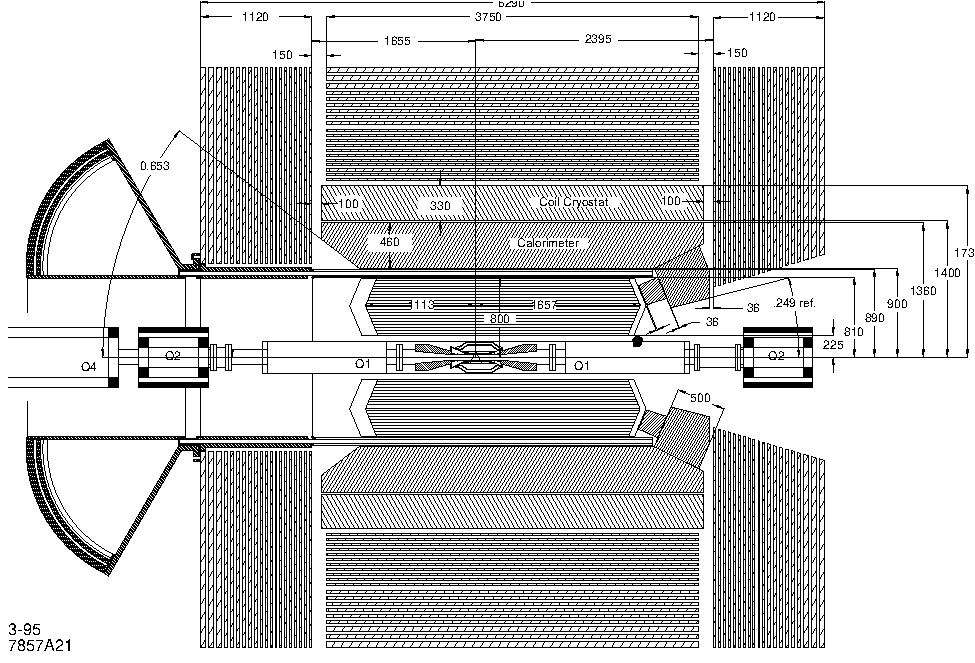
\includegraphics[width=0.7\textwidth]{figs/babar_detector_view.pdf}
    \caption{
        View of the \BaBar/ detector.
        Extracted from \cite{Boutigny:1995ib}.
    }
    \label{fig:babar_detector_view}
\end{figure}

% Talk about BaBar being 4 pi
In $e^- e^+$ detectors, $b \bar{b}$ is produced at all solid angles with
non-negligible probability \cite{Boutigny:1995ib,McGregor:2008ek}, thus the
detector needs to cover almost all solid angles (a $4\pi$ detector).
Indeed, \BaBar/ has tracking coverage of 0.92, namely 92\% of the $4\pi$ solid
angle.

% Talk about tracking and calorimeters
$B$ physics requires excellent vertex resolution and tracking, because the two
$B$ mesons produced by \Y4S/ must be reliably separated.
\BaBar/ has excellent tracking for charged particles, and sufficient spatial
and energy resolution in the electromagnetic calorimeter to reconstruct the
momenta of neutral particles \cite{Bauer:2005} with adequate precision.

\input{include/detectors/01-belle.tex}
\input{include/detectors/02-lhcb.tex}


\section{Review of previous measurements}

\subsection{2013 \BaBar/ $R(D^{(*)})$}
% 2015 BELLE (also hadronic tag)
% BELLE semileptonic tags

\subsection{2016 LHCb $R(D^{*})$}

\subsection{recent measurements from LHCb (forgot the decay channels)}
%2018 LHCb hadronic decay of Tau -> 3* Pi R(D*)


\section{Outlook for LHCb Run 2 measurements}
%\subsection{Current progress}

%\subsection{Expected improvements}

%\subsection{possible drawbacks}
% Remember: Run 2 supposedly has better pile-ups.

\vspace{5em}
\printbibliography
\end{document}
